\section{Progettazione}
\label{progettazione}

\subsection{Database}
\label{progettazione-database}
Il database di appoggio per i contenuti del sito si articola in quattro tabelle. 

La tabella \textit{Utenti} memorizza i dati degli utenti che effettuano la registrazione sul sito; vi appartengono sia gli utenti autenticati che gli utenti amministratori, questi ultimi distinti dal attributo \textit{Admin}, posto ad 1 se l'utente è amministratore.

La tabella \textit{Opere} contiene i dati relativi alle opere presentate nel sito. Di ognuna vengono presentati i dati tecnici, la descrizione e se si tratta di un prestito o di un pezzo permanente della collezione; a questa tabella appartengono sia \textit{dipinti} che \textit{sculture}. Se fosse necessario, in futuro, prevedere altri tipi di opere artistiche, sarebbe sufficiente aggiungere elementi all'attributo "stile" e gli eventuali attributi specifici del nuvo tipo introdotto.

La tabella \textit{Eventi} contiene i dati relativi agli eventi organizzati dal museo. Di ognuno sono riportati i dati logistici e la descrizione; a questa tabella appartengono sia le \textit{conferenze}, previste anche in cicli, che le \textit{mostre}. Se in futuro venissero programmati eventi di altro tipo, per memorizzarli basterebbe aggiungerne la tipologia all'omonimo attributo della tabella, insieme adf altri evenutali attributi specifici dell'evento organizzato.

Infine, la tabella \textit{Recensione} tiene traccia delle recensioni inserite nel sito dagli utenti autenticati. Poiché è previsto che un utente possa modificare una recensione precedentemente inserita, ne viene mantenuta la data di utlima modifica.

\textit{Utenti} è in relazione con le altre tre classi: di ciascun tipo di contenuto previsto, infatti, si memorizza l'utente che ha effettuato l'inserimento. Per \textit{Opere} ed \textit{Eventi} si tratta sempre di un \textit{utente amministratore}, per le recensioni è sempre un \textit{utente autenticato}.

\begin{center}
	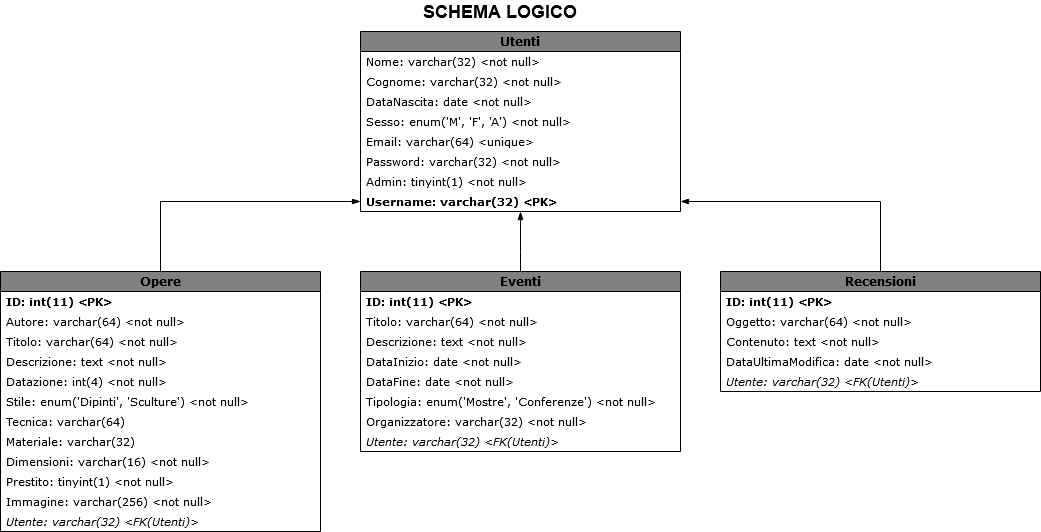
\includegraphics[width=\textwidth]{img/SchemaLogico}
	\captionof{figure}{Schema logico del database del museo \textit{TecArt}}
\end{center}


\subsection{Accessibilità e usabilità}
\label{progettazione-accessibilità-usabilità}


\subsection{\textit{Layout}}
\label{progettazione-layout}
Per la scelta del design delle pagine, l'obiettivo è l'adattabilità al maggior numero possibile di dispositivi, indipendentemente dalle dimensioni dello schermo o dal supporto usato dall'utente. Si è puntato poi ad avere una struttura ordinata, leggera e di immediata comprensione e memorizzazione, al fine di rendere la navigazione semplice e intuitiva.
Per soddisfare queste esigenza è stato scelto il "\textit{layout} a tre pannelli". Come da struttura standard, questo tipo di layout divide la schermata in tre settori: \textit{header} che deve contenere la rispota alla domanda "dove mi trovo?"; \textit{menu}, che deve contenere la rispota alla domanda "dove posso andare?"; \textit{content}, che deve contenere la rispota alla domanda "cosa c'è nella pagina?".
\begin{itemize}
	\item \textit{Header:} su desktop, tablet e mobile occupa la fascia superiore della finestra ed è ampio quanto tutta la schermata. Riporta il nome del sito, il menu per l'accesso all'aera personale e la barra di ricerca. Nella parte più bassa contiene il \textit{breadcrumb}, che indica il percorso fatto dal visitatore all'interno del sito per arrivare alla pagina corrente. Per permettere agilmente all'utente di tornare alla pagine visitate in precedenza, il \textit{breadcrumb} si compone dei link delle pagine corrispondenti. 
	\item \textit{Menu}: riporta i link alle pagine principali del sito, contenenti tutte le informazioni rilevanti per la più ampia categoria di utenti.
	\item \textit{Content}: presenta il contenuto effettivo della pagina.
\end{itemize}
Nella parte più bassa della finestra, simmetricamente all'\textit{header}, si trova il \textit{footer}, che riporta le immagini certificanti la validazione, alcuni dettagli didattici e gli autori del sito. \\\\

In base alle dimensioni della finestra, questi elementi vengono visualizzati in modo diverso. A seguire, un esempio di design per i formati \textit{mobile}, \textit{tablet} e \textit{desktop}.

\begin{center}
	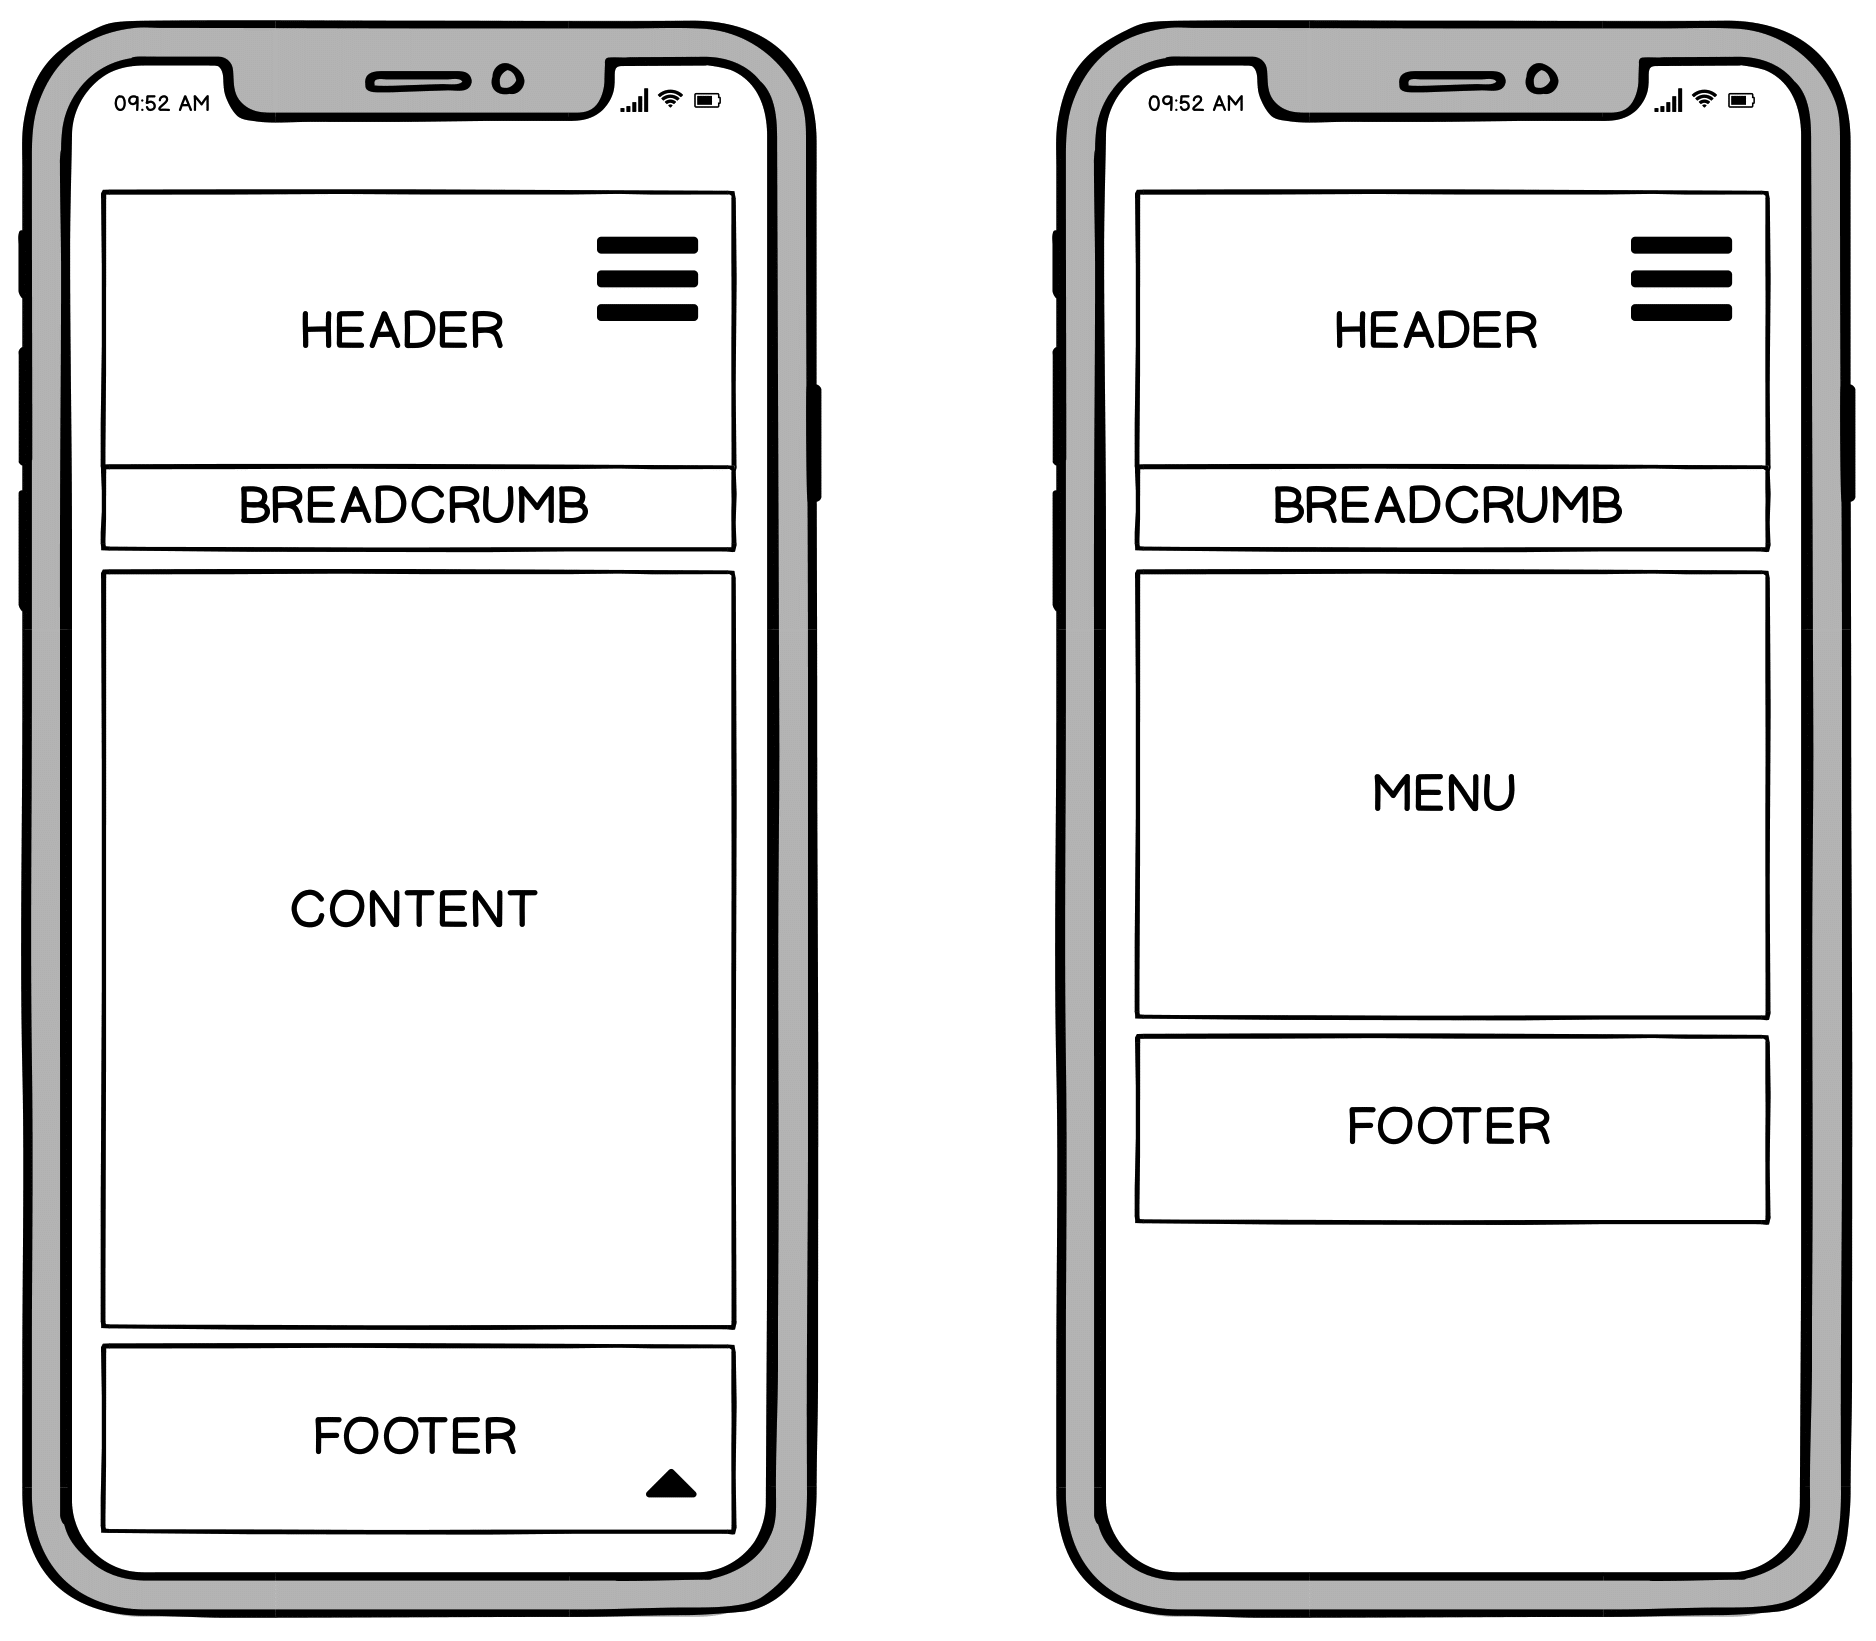
\includegraphics[scale=0.2]{img/Mobile}
	\captionof{figure}{\textit{Layout mobile} con \textit{menu} nascosto (a sinistra) e visibile (a destra)}
\end{center}

\begin{center}
	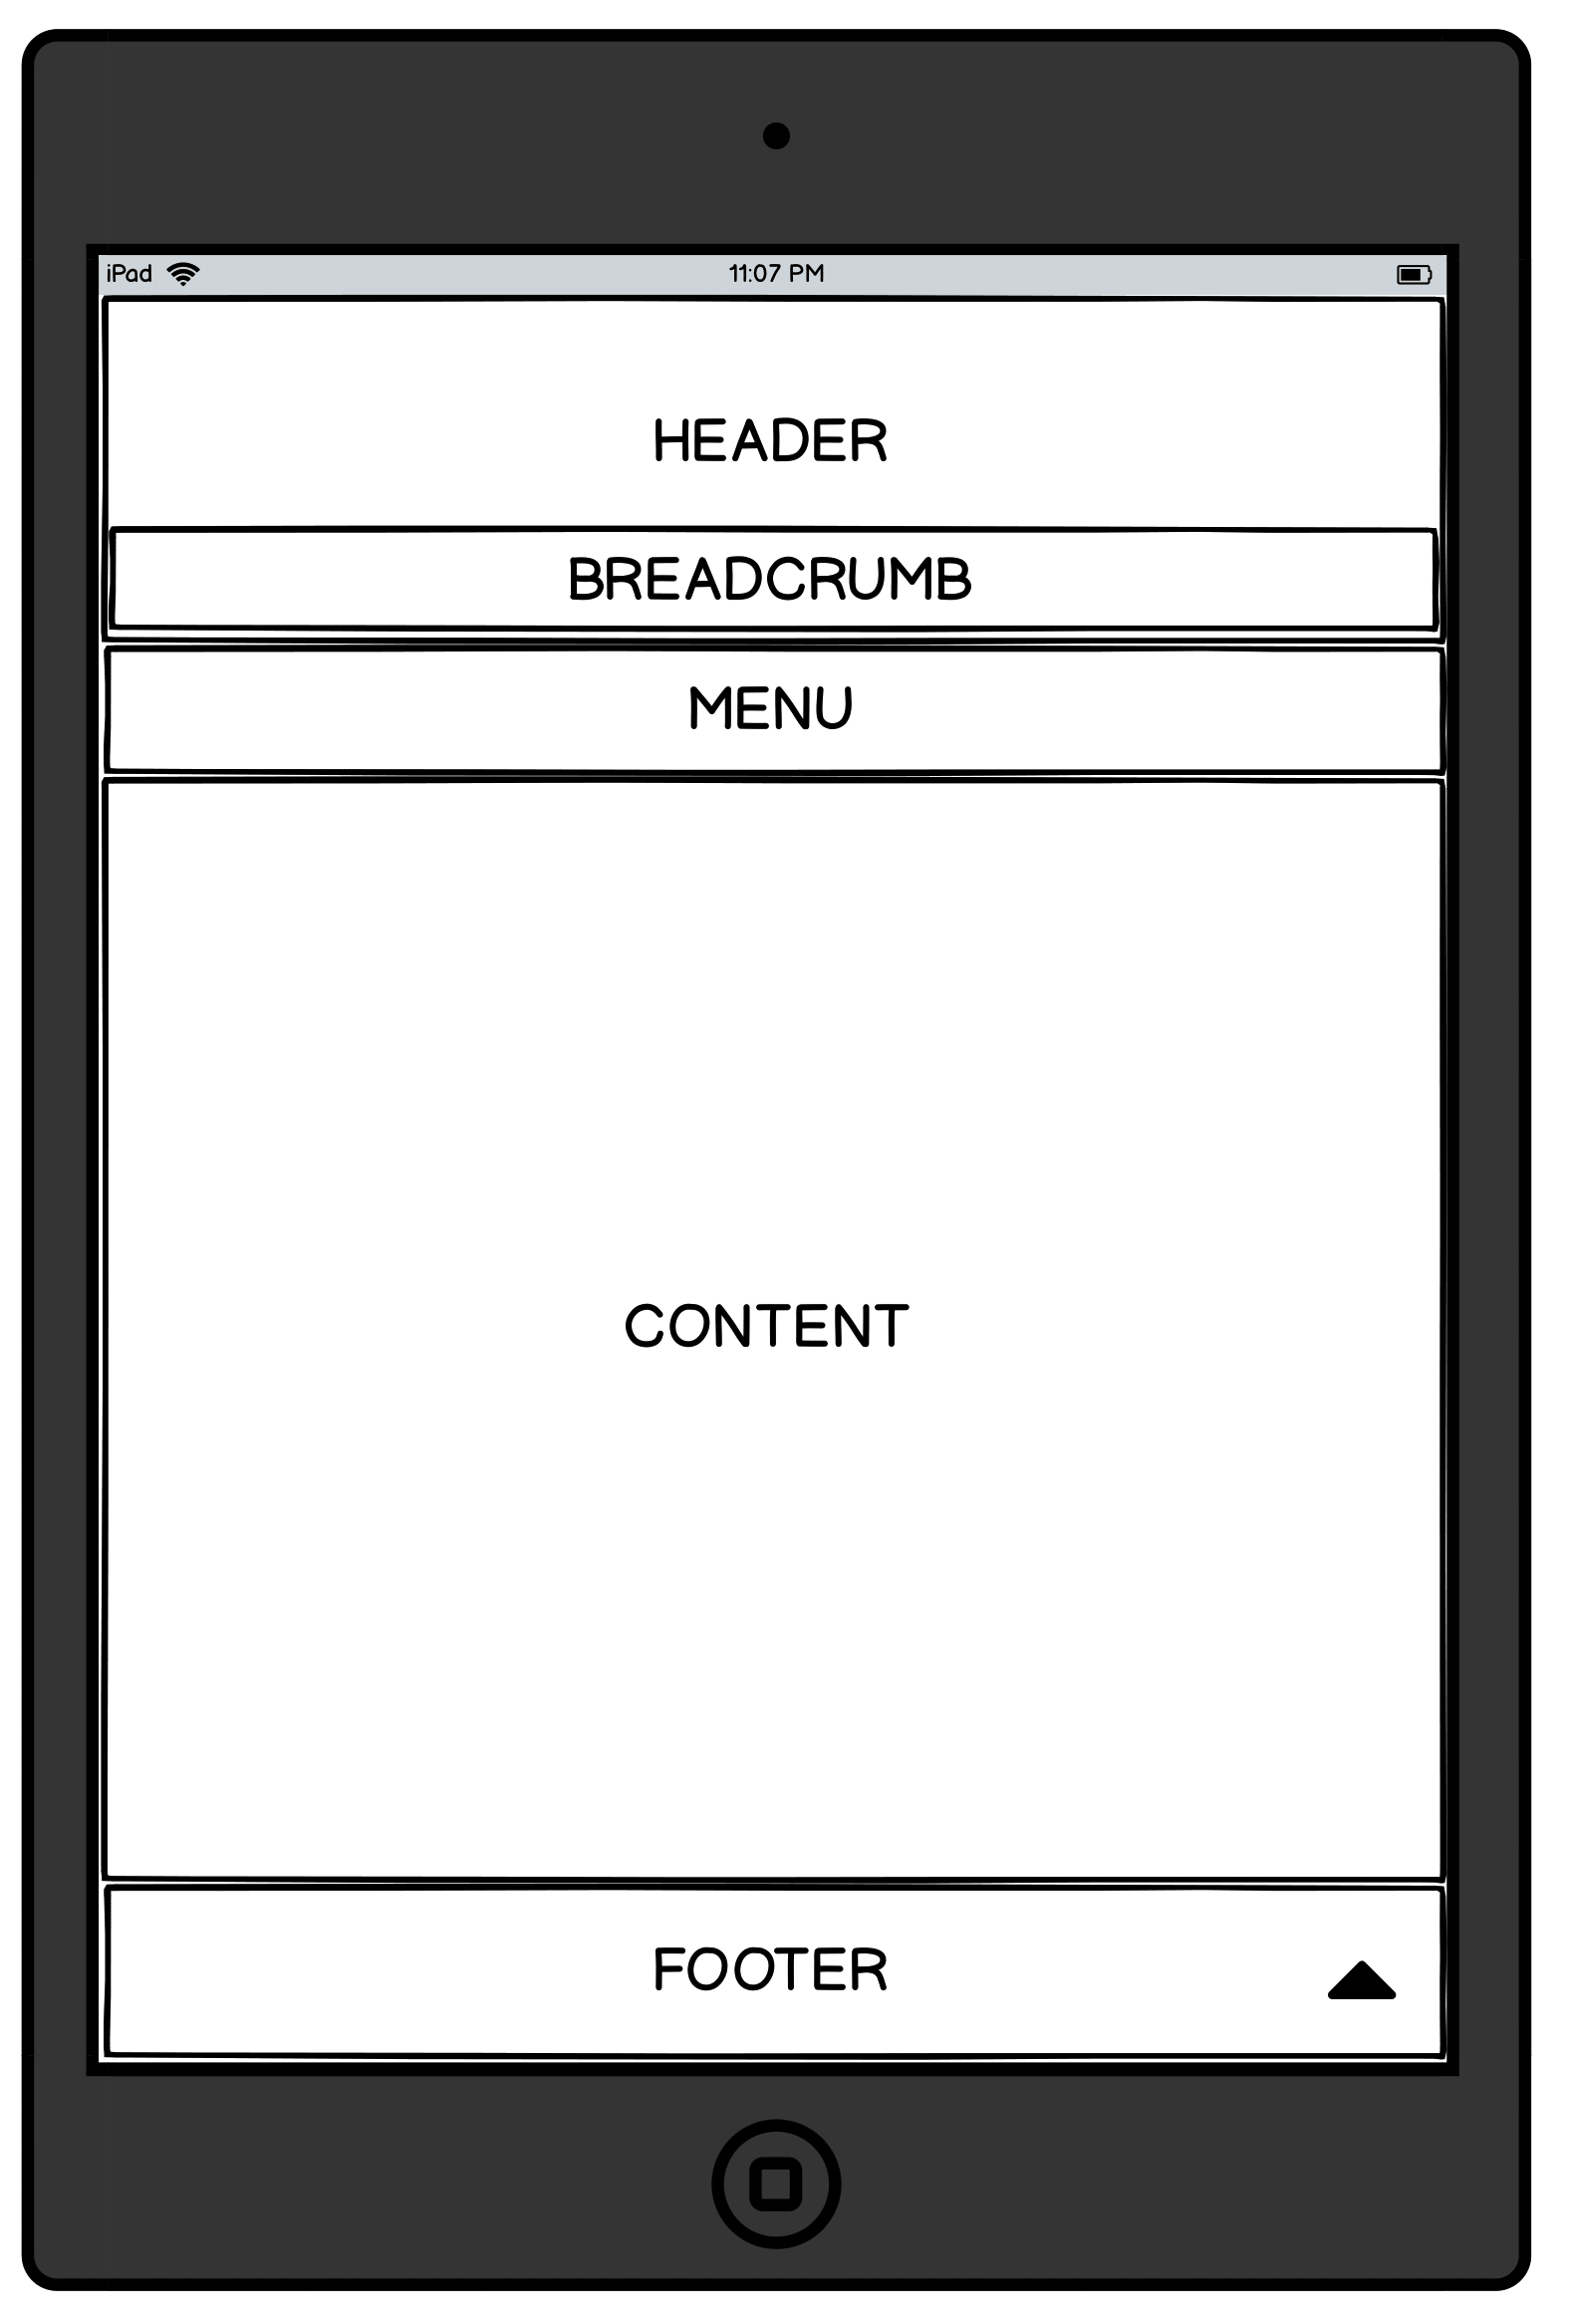
\includegraphics[scale=0.15]{img/Tablet}
	\captionof{figure}{\textit{Layout tablet}}
\end{center}

\begin{center}
	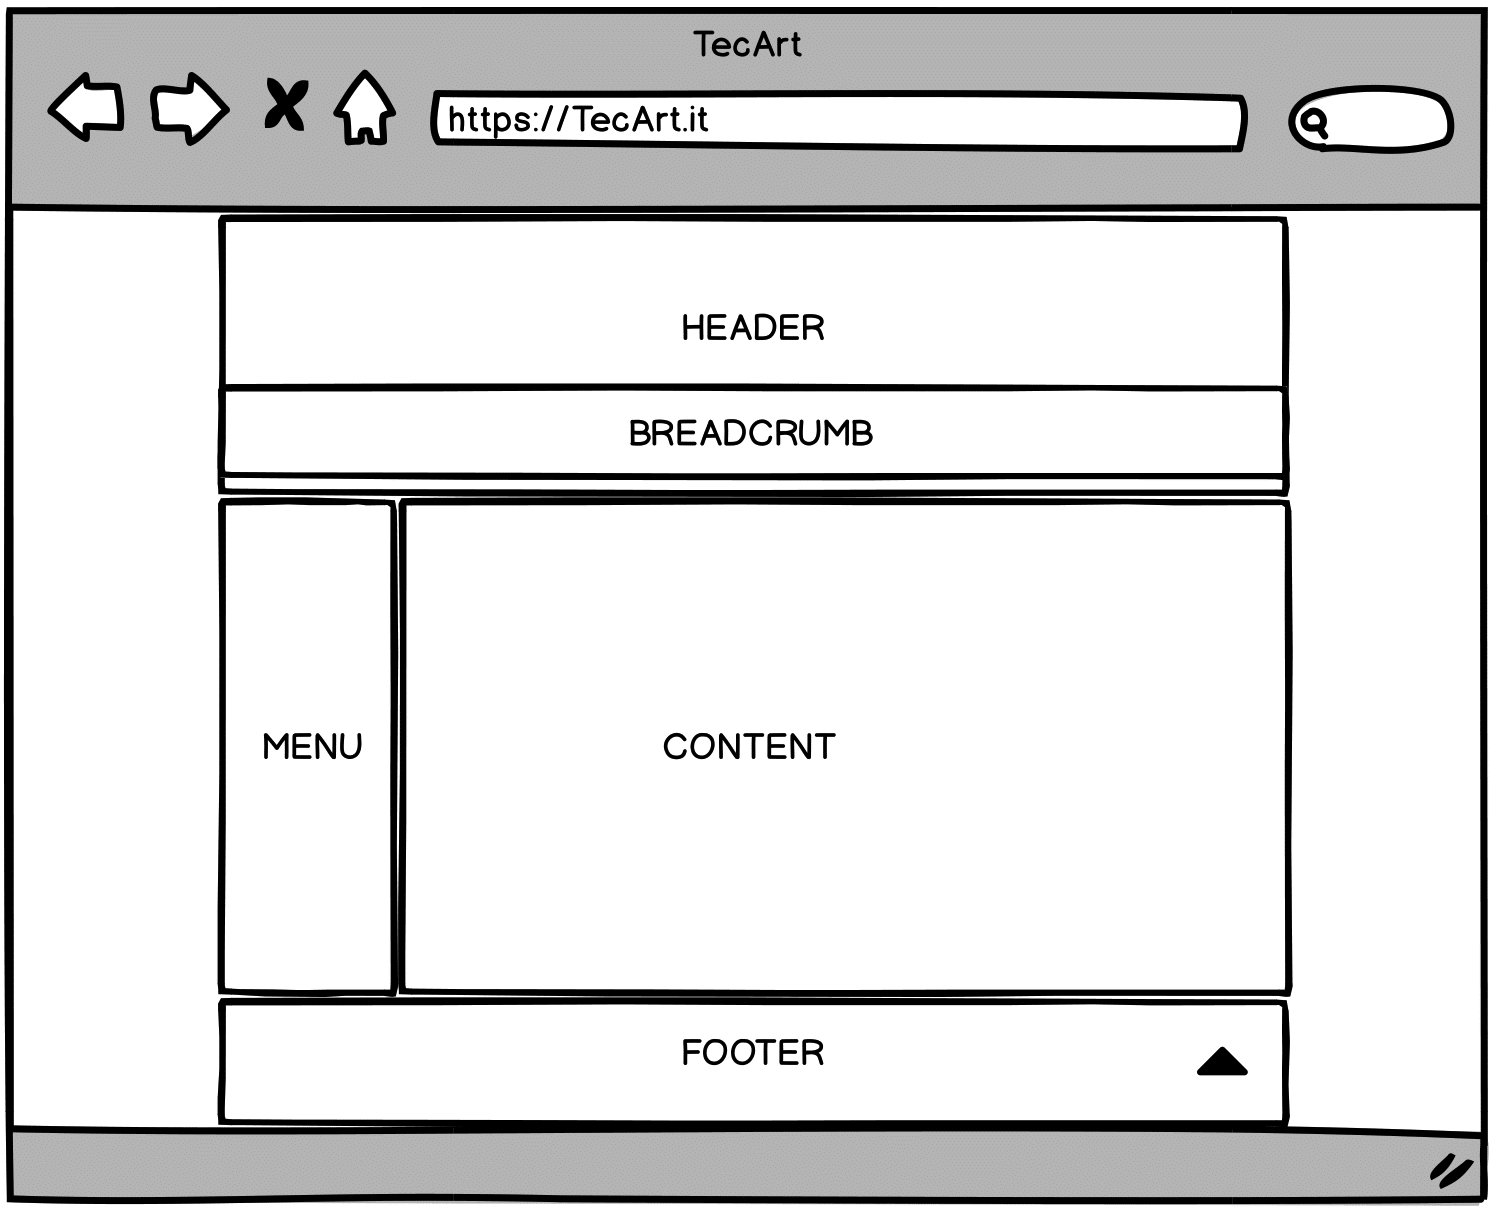
\includegraphics[width=\textwidth]{img/Desktop}
	\captionof{figure}{\textit{Layout desktop}}
\end{center}
